\section{Sistema de Aumento de Estabilidade}

\par Com o objetivo de aumentar o coeficiente de amortecimento do Rolamento Holandês para $\xi > 0.6$ procedeu-se à criação de um Sistema de Aumento de Estabilidade. Procedeu-se, inicialmente, à modelação de um sistema SISO, que permitisse relacionar a razão de guinada com a deflexão do rudder.

    \begin{equation}
    \delta_R = \delta_r^{0} - K_rr
\end{equation}

\begin{equation}
    \frac{r(s)}{\delta_R(s)} = \frac{0.4387s^3 + 0.3838s^2 + 0.0635s + 0.0447}{s^4 + 1.0777s^3 + 0.9023s^2 + 0.5713s - 0.0043}
\end{equation}

\begin{figure}[htbp]
    \centering
    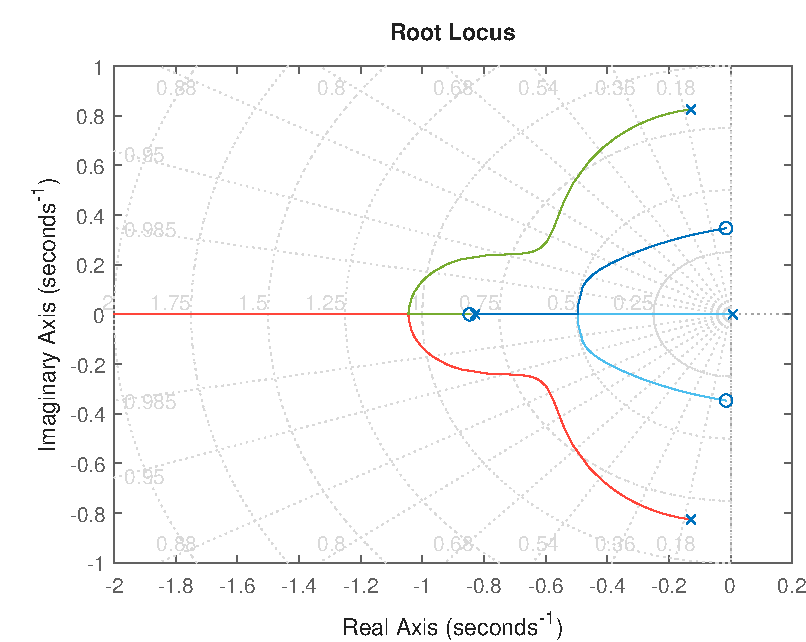
\includegraphics[width=0.45\textwidth]{Body/Images/root_locus.pdf}
    \caption{Root locus do sistema SISO}
    \label{fig:root_locus}
\end{figure}